\chapter{教学实验与计算实验}
\label{chap:e26}

\begin{chapteropening}
到这里为止，我们已经把整套语言搭好了：光子的到达是随机点过程（第 \ref{chap:e03} 章），热光会\textbf{聚束}、相干光不聚束（第 \ref{chap:e08} 章），两台望远镜之间的空间相干度就是天体亮度分布的可见度（第 \ref{chap:e10}、\ref{chap:e11} 章），而有些参数的信息根本不在你最习惯看的那张图里（第 \ref{chap:e12} 章）。这些道理讲一遍是一回事，\textbf{亲手把它算出来、看见它、并且知道哪里会骗你}，是另一回事。本章就是那间实验室。我们不给出一堆可以直接跑的代码，而是把每一个关键概念拆成一条\textbf{可复算的实验链}：从一张模拟的光子事件表出发，看它怎样变成统计量，统计量怎样进入物理模型，模型的误差又怎样反过来逼你重新设计实验。沿途你会用模拟数据亲眼验证泊松分布和聚束、数值演示 SPADE 如何越过瑞利极限、拟合均匀圆盘和双星的可见度，最后把这些零件拼成一个 Type Ia 超新星测距的玩具模型。每个实验都配一句"常见的坑"，因为在这一行里，一条太漂亮的曲线往往不是好消息，而是一个还没被发现的错误。
\end{chapteropening}

\section{事件表：所有计算实验共用的底稿}
\label{sec:e26-eventtable}

先建立画面。做这一章所有实验的起点，都是一张\textbf{事件表}（event table）——它不是什么高深的数据结构，就是一张表，每一行记一个光子：它什么时候到（时间戳 \(t_i\)）、落在哪个探测器或哪个通道、偏振是什么、以及一个"质量标记"\(q_i\) 说明这个光子可不可信（是不是落在死时间附近、有没有被云挡、电子学有没有饱和）。第 \ref{chap:e13} 章讲过为什么要这么存：一旦你先把光子按时间粗分箱、连成一条平滑的\textbf{光变曲线}（light curve），你就再也无法回头重新选时间窗、重新按偏振或能道筛选、重新做时间平移的背景估计了。分箱是一种\textbf{有损压缩}。事件表则把光场的随机性原封不动地留在硬盘上。

真实的光子计数仪器正是这么工作的。AQuEye、IquEye 这类设备把每个光子都保留成一个时间标签，时间分辨率可到几十皮秒，绝对时间靠 GPS 或原子钟约束到纳秒乃至亚纳秒；像 Timepix 这样的像素计数芯片还能让每一行同时带上空间位置和能量信息 \citep{2016SPIE.9907E..0NZ,2015SPIE.9504E..0CZ,2007NIMPA.581..485L}。所以本章的第一条纪律是：\textbf{实验从事件表开始，不从光变曲线开始}。

如果你确实只关心光变曲线，那也很简单——把事件表按时间 bin 投影一下就行：
\begin{equation}
  n_k=\sum_i \mathbf 1\!\big(t_i\in[t_k,\,t_k+\Delta t)\big)\,\mathbf 1\!\big(q_i=1\big).
  \label{eq:e26-binned-count}
\end{equation}
\begin{formulaexplain}
\(n_k\) 是第 \(k\) 个时间箱里"通过质量筛选"的光子数。两个指示函数 \(\mathbf 1(\cdot)\) 像两道闸门：第一道检查光子到达时刻是否落进这个箱，第二道检查这个光子质量是否合格（\(q_i=1\) 才放行）。求和就是数一数有几个光子同时通过两道闸门。
\end{formulaexplain}
逐个符号落实单位与量纲。\(n_k\) 是一个纯计数，没有量纲；\(\Delta t\) 是箱宽（单位 s），桌面实验常取纳秒到毫秒，天文计时可以从纳秒一路到分钟；\(\mathbf 1(A)\) 是指示函数，条件 \(A\) 成立取 1、否则取 0。想把它变成光子率，只需 \(r_k=n_k/\Delta t\)，单位是 \(\mathrm{s^{-1}}\)。这里已经埋了一个坑：当每箱平均只有几个到几十个光子时，计数涨落是泊松型的，\textbf{不能}随手用对称的高斯误差棒替代；要等到 \(n_k\gtrsim30\)，高斯近似才大致可用。式 \eqref{eq:e26-binned-count} 看起来平淡，但它是本章每一个实验的第一步：先有事件表，再决定投影成什么。

\begin{figure}[tbp]
\centering
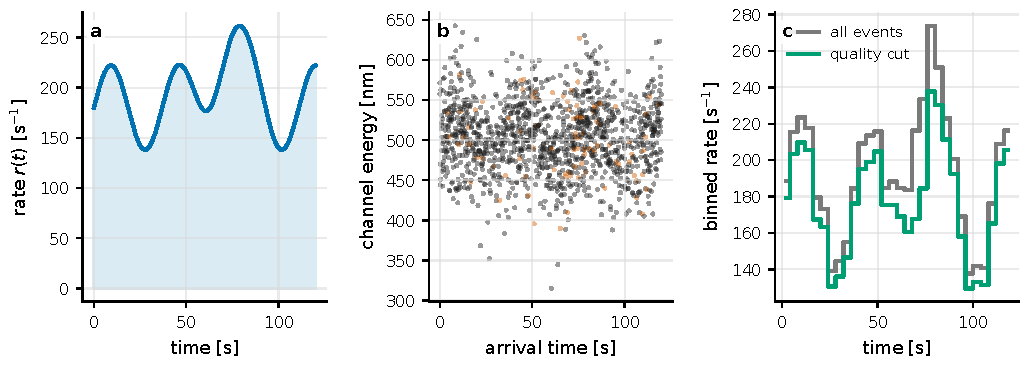
\includegraphics[width=0.96\linewidth]{figures/generated/chapter_20/ch20_event_table_simulation.pdf}
\caption{用非齐次泊松过程生成的模拟事件表。左图是输入光子率 \(r(t)\)；中图保留每个光子的到达时间、等效波长通道和质量标记；右图把事件表投影成光变曲线，并显示质量筛选的影响。事件表比光变曲线多留了通道与质量信息，因此同一份数据还能重新拿去做相关、偏振或能谱分析。}
\label{fig:e26-eventtable}
\end{figure}

\section{第一个计算实验：造一张事件表，验证泊松与散粒噪声}
\label{sec:e26-poisson}

第一个实验的目标最朴素，却最重要：\textbf{亲手造出一张符合泊松统计的事件表，再用它把泊松统计验证回来}，从而彻底吃透第 \ref{chap:e03} 章的散粒噪声。

先说"怎么造"。若光子率恒定为 \(r\)，最省事的办法是利用泊松过程的一个性质：相邻两个光子的时间间隔服从指数分布，\(P(\Delta t)=r\,e^{-r\Delta t}\)。于是从一个均匀随机数 \(u\in(0,1)\) 取 \(\Delta t=-\ln(u)/r\)，一个接一个累加，就得到一串到达时刻。如果率是随时间变的 \(r(t)\)（比如图 \ref{fig:e26-eventtable} 左图那种起伏），就用\textbf{稀释法}（thinning）：先按一个高于所有时刻的常率 \(r_{\max}\) 生成候选光子，再对每个候选以概率 \(r(t_i)/r_{\max}\) 独立地"留下或丢弃"。留下的那些，就是非齐次泊松过程的一次真实实现。这个方法的好处是它逼你把"随机性从哪来"想清楚，而不是调一个黑箱函数。

现在验证。恒定率下，落在长度 \(\Delta t\) 的箱里的光子数 \(N\) 服从泊松分布，这是第 \ref{chap:e03} 章的已知结果，直接点名使用：
\begin{equation}
  P(N)=\frac{\mu^{N}}{N!}\,e^{-\mu},\qquad \mu=r\,\Delta t .
  \label{eq:e26-poisson-pmf}
\end{equation}
\begin{formulaexplain}
\(P(N)\) 是一个箱里恰好数到 \(N\) 个光子的概率，\(\mu\) 是这个箱的\textbf{平均}光子数（等于率乘箱宽）。泊松分布只由一个参数 \(\mu\) 决定，它同时是均值也是方差——这是它最好用、也最好检验的性质。
\end{formulaexplain}
落实符号：\(N\) 是无量纲计数，\(\mu=\bar N\) 是无量纲的平均计数，\(r\) 单位 \(\mathrm{s^{-1}}\)，\(\Delta t\) 单位 s。泊松分布最能被一眼验证的地方，是它的均值与方差\textbf{相等}。我们把这一点写成一个可以直接从数据算的检验量——\textbf{法诺因子}（Fano factor）：
\begin{equation}
  F=\frac{\operatorname{Var}(N)}{\langle N\rangle}\;\xrightarrow[\text{泊松}]{}\;1 .
  \label{eq:e26-fano}
\end{equation}
\begin{formulaexplain}
\(\langle N\rangle\) 是各箱计数的样本均值，\(\operatorname{Var}(N)\) 是它们的样本方差。法诺因子 \(F\) 就是两者之比。纯泊松（相干光、散粒噪声主导）给出 \(F=1\)；聚束的热光会让 \(F>1\)，反聚束的非经典光会让 \(F<1\)。
\end{formulaexplain}
为什么泊松的方差恰好等于均值？这不是巧合，值得当场点名推一遍。由式 \eqref{eq:e26-poisson-pmf}，
\[
  \langle N\rangle=\sum_{N=0}^{\infty}N\,\frac{\mu^N}{N!}e^{-\mu}
  =\mu\,e^{-\mu}\sum_{N=1}^{\infty}\frac{\mu^{N-1}}{(N-1)!}
  =\mu\,e^{-\mu}\,e^{\mu}=\mu,
\]
其中用到了\textbf{几何级数式的指数展开} \(\sum_{m\ge0}\mu^m/m!=e^{\mu}\)（把 \(m=N-1\) 换元即得）。同理算二阶阶乘矩：
\[
  \langle N(N-1)\rangle=\sum_{N=0}^{\infty}N(N-1)\frac{\mu^N}{N!}e^{-\mu}
  =\mu^2 e^{-\mu}\sum_{N=2}^{\infty}\frac{\mu^{N-2}}{(N-2)!}=\mu^2 .
\]
于是 \(\langle N^2\rangle=\langle N(N-1)\rangle+\langle N\rangle=\mu^2+\mu\)，代入方差定义：
\[
  \operatorname{Var}(N)=\langle N^2\rangle-\langle N\rangle^2=(\mu^2+\mu)-\mu^2=\mu .
\]
方差等于均值，一步不跳。这就是散粒噪声那句名言"\(\sigma_N=\sqrt{\bar N}\)"的来处，也是式 \eqref{eq:e26-fano} 里 \(F\to1\) 的根据。

数量级落地：若你造的事件表平均率 \(r=5\times10^{5}\,\mathrm{s^{-1}}\)、箱宽 \(\Delta t=1\,\mathrm{ms}\)，则每箱 \(\mu=500\) 个光子，相对涨落 \(1/\sqrt{\mu}\simeq4.5\%\)；把箱宽缩到 \(1\,\mu\mathrm{s}\)，\(\mu=0.5\)，绝大多数箱是空的，法诺检验要靠大量箱的统计才稳。\textbf{常见的坑}：如果你算出 \(F\) 明显偏离 1，先别急着宣布看到了非经典光——更可能是探测器\textbf{死时间}（dead time）在作怪。死时间会在一个光子之后短暂"致盲"，压低紧挨着的计数，从而人为地把方差压到均值以下（\(F<1\)），伪装成反聚束。所以这个最基础的实验，其实是在教你分辨"物理"和"仪器"。

\section{桌面 HBT：从随机符合里"看见"聚束}
\label{sec:e26-hbt}

第二个实验把泊松推进到\textbf{二阶}：用一束光、一个分束器、两个探测器，做一次桌面版的汉伯里·布朗–特维斯（Hanbury Brown--Twiss, HBT）实验，亲手测出 \(g^{(2)}(\tau)\)，验证第 \ref{chap:e08} 章的聚束 \citep{1956Natur.178.1046H,1957RSPSA.242..300B,1963PhRv..130.2529G}。

先要画面。两路强度各自都在随机跳动，凭什么零延迟附近会比别处多一点"共同的"起伏？把热光（或旋转毛玻璃造出的\textbf{伪热光}, pseudothermal light）想成许多相位随机的模式叠加，它的瞬时强度并不平，而是忽高忽低。在同一个\textbf{相干时间} \(\tau_c\) 之内，这一次强度涨落是被两个探测器\textbf{共享}的——强度高的那一瞬，两边同时更容易各接到一个光子，于是"符合"（coincidence）在 \(\tau=0\) 附近增多。激光是例外：它每个模式相位锁定，强度平得像一潭死水，所以 \(g^{(2)}(0)\simeq1\)，不聚束 \citep{1991PhRvL..67.1426N,1999PhRvA..60..674B,2024arXiv240418606N}。

怎么从事件表把它算出来？做法是数\textbf{符合对}并归一化。把两路事件表按时间差 \(\tau=t_j^{(2)}-t_i^{(1)}\) 统计成一个延迟直方图 \(H(\tau)\)，再除以一个"本该如此"的随机基线：
\begin{equation}
  \hat g^{(2)}(\tau)=\frac{H(\tau)}{H_{\rm bg}(\tau)},\qquad
  H_{\rm bg}\simeq R_1 R_2\,T\,\Delta\tau .
  \label{eq:e26-g2-estimator}
\end{equation}
\begin{formulaexplain}
\(H(\tau)\) 是时间差落在第 \(\tau\) 个延迟箱里的光子对数目。\(H_{\rm bg}\) 是"如果两路完全独立"时该有的偶然符合数：两路率 \(R_1,R_2\) 相乘、乘总时长 \(T\)、再乘延迟箱宽 \(\Delta\tau\)。相除就把仪器的绝对计数抵掉，只留下\textbf{相对}于随机符合的超额。
\end{formulaexplain}
落实符号：\(R_1,R_2\) 是两路单计数率（\(\mathrm{s^{-1}}\)），\(T\) 是总积分时间（s），\(\Delta\tau\) 是延迟箱宽（s），\(H,H_{\rm bg}\) 都是无量纲计数。分母 \(H_{\rm bg}\) 有一个更靠谱的实测版本：把第二路整体\textbf{时间平移}一个远大于 \(\tau_c\) 的量再数一遍符合——那时物理相关早已消失，剩下的纯是偶然，这就是\textbf{time-shift 背景}。用它归一化，能自动吸收慢漂移。

数量级要让人心里有底。取 \(R_1=R_2=5\times10^{5}\,\mathrm{s^{-1}}\)、\(T=300\,\mathrm{s}\)、\(\Delta\tau=0.5\,\mathrm{ns}\)，则每个延迟箱的随机符合约
\[
  H_{\rm bg}\simeq (5\times10^5)^2\times300\times(0.5\times10^{-9})\approx3.75\times10^{4}\ \text{对/箱}.
\]
这些对数本身是泊松涨落的，散粒相对误差约 \(1/\sqrt{H_{\rm bg}}\simeq5\times10^{-3}\)。于是一个 \(g^{(2)}-1\sim10^{-2}\) 的峰在桌面上抬头可见——而这正是问题所在。

\begin{figure}[tbp]
\centering
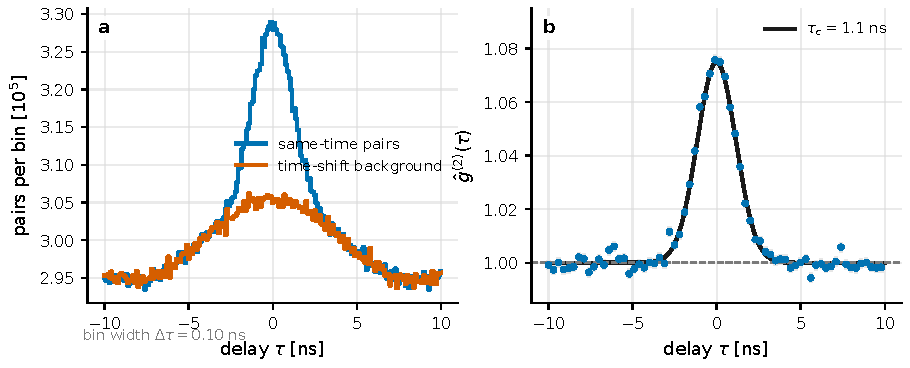
\includegraphics[width=0.96\linewidth]{figures/generated/chapter_20/ch20_hbt_lab_histogram.pdf}
\caption{桌面 HBT 的延迟直方图。左图比较同时时间轴上的"对/箱"与 time-shift 背景；慢漂移会同时出现在两条曲线里，因此被归一化抵掉。右图用背景直方图归一化后得到 \(\hat g^{(2)}(\tau)\)，零延迟附近的峰宽由光源相干时间与探测器响应共同决定。}
\label{fig:e26-hbt}
\end{figure}

\textbf{最要命的坑：对比度稀释。}真实仪器测到的不是理想 \(g^{(2)}\)，而是它被探测器时间响应\textbf{卷积}后的样子。若相干时间 \(\tau_c\) 远小于电子学响应宽度或延迟箱宽 \(\Delta\tau\)，热光本该到 2 的峰会被稀释，观测对比度近似按 \(\tau_c/\Delta\tau\) 缩小。算给你看：一片中心 \(416\,\mathrm{nm}\)、带宽 \(\Delta\lambda=13\,\mathrm{nm}\) 的窄带滤光片，带宽换算 \(\Delta\nu\simeq c\,\Delta\lambda/\lambda^2\approx2.3\times10^{13}\,\mathrm{Hz}\)，相干时间 \(\tau_c\simeq1/\Delta\nu\approx4\times10^{-14}\,\mathrm{s}\)；用几纳秒的电子学去采样，对比度被压到 \(\tau_c/\Delta\tau\sim10^{-5}\) 量级。这就是为什么桌面上若看到一个又高又漂亮的峰，你的第一反应\textbf{不应该}是高兴，而应该是追问：它到底来自单模热光，还是电子学串扰、光源慢漂移、或者归一化选得太巧？VERITAS、MAGIC、Asiago 的强度干涉分析无一例外都要显式处理这份稀释、背景与死时间账本 \citep{2009A&A...508..531N,2020NatAs...4.1164A,2024MNRAS.529.4387A,2017MNRAS.472.4126G}。这也顺带解释了下一节的分工：桌面能看见的 \(10^{-2}\) 峰，和天文上要抠的 \(10^{-5}\) 峰，差着五个数量级。

\section{从桌面到长基线：模拟并拟合均匀圆盘的可见度}
\label{sec:e26-disk}

把 HBT 从桌面搬到\textbf{两台望远镜}之间，它就成了强度干涉仪（第 \ref{chap:e10} 章）。物理没变——仍然是比较两路强度起伏是否同步——但现在两台望远镜看的是同一颗\textbf{有角大小}的星。基线越长，两个孔径看到的相干涨落越不一样，零延迟峰就越低。这份"随基线下降"的曲线，正是天体亮度分布的可见度。

第 \ref{chap:e08} 章的 Siegert 关系告诉我们，二阶相关的超额等于一阶相干度的模平方；第 \ref{chap:e10} 章的 van Cittert--Zernike 定理又告诉我们，两台望远镜之间的一阶空间相干度 \(\gamma_{12}\) 就是天体归一化亮度分布的傅里叶变换，即可见度 \(V\)。把两者接起来，实验上从数据估计 \(|V|^2\) 的流程是这样的：每条基线 \(b\) 先给出零延迟的过量相关 \(\hat c_b=\hat g^{(2)}_b(0)-1\)，再用当夜的标定星（或实验室标定）测得的仪器对比度 \(\hat\beta_b\) 去除：
\begin{equation}
  \widehat{|V_b|^2}=\frac{\hat c_b}{\hat\beta_b}.
  \label{eq:e26-v2-estimator}
\end{equation}
\begin{formulaexplain}
\(\hat c_b\) 是基线 \(b\) 测到的零延迟相关超额，\(\hat\beta_b\) 是同一条基线的仪器对比度（把时间响应、带宽、偏振选择、效率造成的稀释一并收进去）。两者相除才剥出天体自己的 \(|V_b|^2\)。注意：\(\beta\) 出现在\textbf{分母}，所以它的标定误差会被\textbf{直接放大}进结果。
\end{formulaexplain}
\(\hat c_b\)、\(\hat\beta_b\)、\(|V_b|^2\) 都是无量纲量。若某基线的随机符合数为 \(H_b\)、系统误差暂忽略，则 \(\sigma_{\hat c}\simeq H_b^{-1/2}\)；可一旦真实对比度小到 \(\beta\sim10^{-5}\)，同样的 \(\sigma_{\hat c}\) 就被放大成 \(\sigma_{|V|^2}\simeq\sigma_{\hat c}/\beta\)。\textbf{教学模拟的坑正在这里}：为了让信号在图上看得见，你会忍不住把 \(\beta\) 取到 \(0.05\) 这种"友好"的值，于是得到一个假装很干净的 \(g^{(2)}\) 峰；但真实天文 \(|V|^2\) 的精度，仍然由那个 \(10^{-6}\)–\(10^{-5}\) 的真实对比度、随机符合数和系统地板决定。做模拟时把这个放大因子写在报告最显眼处，是基本诚实。

现在造数据、做拟合。最常用的源模型是\textbf{均匀圆盘}（uniform disk），它的可见度是第 \ref{chap:e11} 章的已知结果，直接点名：
\begin{equation}
  V(B_\perp)=\frac{2J_1(x)}{x},\qquad
  x=\frac{\pi\,\theta\,B_\perp}{\lambda},
  \label{eq:e26-uniform-disk}
\end{equation}
\begin{formulaexplain}
\(V\) 是可见度，\(J_1\) 是一阶贝塞尔函数，\(x\) 是把角直径、基线、波长揉成的一个无量纲组合。\(x\) 越大（基线越长或星越大），\(V\) 越小；\(2J_1(x)/x\) 在 \(x\to0\) 时趋于 1，第一次归零发生在 \(x=3.8317\)。观测里能拿到的是 \(|V|^2\)，相位信息在强度干涉里丢了符号。
\end{formulaexplain}
逐个落实：\(\theta\) 是角直径（rad，报告里常写 mas 或 \(\mu\mathrm{as}\)），\(B_\perp\) 是投影基线（m），\(\lambda\) 是观测波长（m），\(J_1\) 无量纲。把第一零点 \(x=3.8317\) 代进去，得到最能定角直径的那条基线：
\[
  B_{\rm null}=\frac{3.8317}{\pi}\,\frac{\lambda}{\theta}\approx1.22\,\frac{\lambda}{\theta}.
\]
代真实数字：\(\lambda=416\,\mathrm{nm}\)、\(\theta=1\,\mathrm{mas}=4.85\times10^{-9}\,\mathrm{rad}\)，
\[
  B_{\rm null}\approx1.22\times\frac{416\times10^{-9}}{4.85\times10^{-9}}\ \mathrm{m}\approx105\,\mathrm{m}.
\]
这一个数就解释了整片版图：\(1\,\mathrm{mas}\) 亮星的第一零点落在百米级基线，所以 VERITAS 这类百米级切伦科夫阵列能测亮星角直径；而 Type Ia 超新星那几个 \(\mu\mathrm{as}\) 的角半径，第一零点要退到几十公里以外，只能靠公里级基线。拟合时的\textbf{要点}是：\(|V|^2\) 对 \(\theta\) 最敏感的地方在第一零点附近的陡坡上，所以基线覆盖若全挤在 \(V\approx1\) 的平台区，后验会很宽；把基线铺到零点两侧，角直径才收得紧。

\begin{figure}[tbp]
\centering
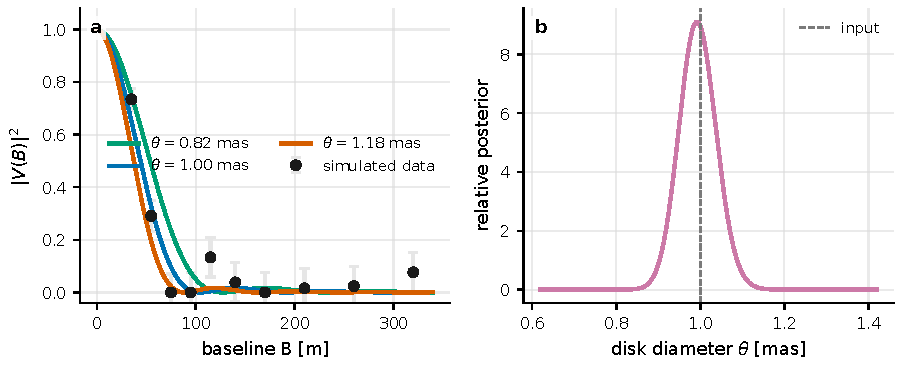
\includegraphics[width=0.96\linewidth]{figures/generated/chapter_20/ch20_uniform_disk_fit.pdf}
\caption{均匀圆盘的强度干涉拟合。左图模拟 \(\lambda=416\,\mathrm{nm}\)、\(\theta=1\,\mathrm{mas}\) 的目标在不同基线上的 \(|V|^2\) 测量，第一零点附近斜率最大、对角直径最敏感。右图把这些数据转成角直径后验，后验宽度由 \(|V|^2\) 误差、基线覆盖和模型假设共同决定。}
\label{fig:e26-disk}
\end{figure}

\section{双星与 uv 覆盖：为什么要多基线、多历元}
\label{sec:e26-binary}

均匀圆盘只有一个参数，双星把故事变有趣：它让你亲眼看到，强度干涉虽然丢了可见度的\textbf{符号}（相位），却仍然保留了随基线振荡的\textbf{空间频率}。两个非相干点源的归一化可见度平方是第 \ref{chap:e10}、\ref{chap:e11} 章的已知结果：
\begin{equation}
  |V(\bm B_\perp)|^2=\frac{1+\rho^2+2\rho\cos\!\big(2\pi\,\bm B_\perp\!\cdot\!\bm s/\lambda\big)}{(1+\rho)^2},
  \label{eq:e26-binary}
\end{equation}
\begin{formulaexplain}
\(\rho=F_2/F_1\) 是伴星与主星的通量比，\(\bm s\) 是两星的角分离向量，\(\bm B_\perp\!\cdot\!\bm s/\lambda\) 是投影到基线方向上的无量纲相位。分子里的余弦项让 \(|V|^2\) 随基线上下振荡，分母 \((1+\rho)^2\) 只是把它归一化到 \(\bm B_\perp\to0\) 时的 1。
\end{formulaexplain}
落实符号与量纲：\(\rho\) 无量纲，\(\bm s\) 是角度向量（rad，报告常用 mas），\(\bm B_\perp\) 单位 m，\(\lambda\) 单位 m，整个 \(\bm B_\perp\!\cdot\!\bm s/\lambda\) 无量纲。看两个极端能体会它在说什么。等亮双星 \(\rho=1\) 时，式 \eqref{eq:e26-binary} 化成 \((1+\cos\phi)/2\)，随相位从 1 一路荡到 0——满调制。若伴星只有主星一成通量 \(\rho=0.1\)，余弦项让 \(|V|^2\) 围绕自己的均值上下摆动，这个\textbf{振荡半幅}为
\[
  \frac{2\rho}{(1+\rho)^2}=\frac{2\times0.1}{1.1^2}\approx0.17,
\]
而摆动的中心（均值）是 \(\dfrac{1+\rho^2}{(1+\rho)^2}=\dfrac{1.01}{1.21}\approx0.835\)。于是 \(|V|^2\) 在均值 \(0.835\) 上下各摆 \(0.17\)，实际是在约 \(0.67\) 到 \(1\) 之间起伏：最大值 \(1\) 出现在 \(\cos\phi=1\)，最小值 \(\dfrac{(1-\rho)^2}{(1+\rho)^2}=\dfrac{0.81}{1.21}\approx0.67\) 出现在 \(\cos\phi=-1\)，峰谷差约 \(0.33\)。伴星越暗，波纹越浅，越考验测量精度。相位也算一个给你看：\(B=180\,\mathrm{m}\)、\(\lambda=500\,\mathrm{nm}\)、分离 \(0.5\,\mathrm{mas}=2.42\times10^{-9}\,\mathrm{rad}\) 时，
\[
  \phi=2\pi\frac{B\,s}{\lambda}=2\pi\times\frac{180\times2.42\times10^{-9}}{500\times10^{-9}}\approx5.5\ \mathrm{rad},
\]
接近一整圈——单条基线上就能看到明显的一个振荡周期。

但一条基线只是 uv 平面上的\textbf{一个点}（第 \ref{chap:e11} 章）。要同时定出分离的大小、方向、通量比和轨道几何，就得铺开 uv 覆盖：多条基线在一个时刻采到不同的 \(\bm B_\perp\)，加上地球自转让每条基线的投影 \(\bm B_\perp(t)\) 在一夜里划出弧线（\textbf{地球自转合成孔径}），多历元又让 \(\bm s(t)\) 随轨道运动扫过不同相位。这就是"多基线、多历元"这句口号的实质：\textbf{用不同的 uv 采样把简并的参数一个个拆开}。\textbf{常见的坑}：若 uv 覆盖只沿一个方向，垂直方向的分离就基本不受约束，拟合会给出一个被拉长的、误导人的误差椭圆——图好看，参数不可信。

\begin{figure}[tbp]
\centering
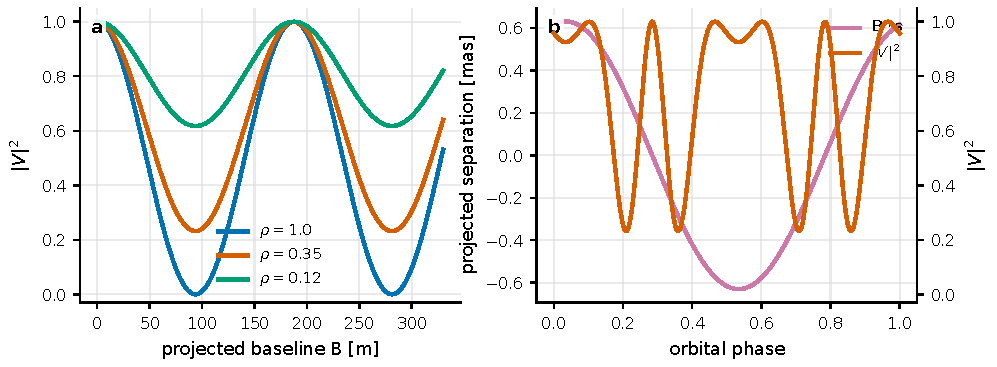
\includegraphics[width=0.96\linewidth]{figures/generated/chapter_20/ch20_binary_visibility.pdf}
\caption{双星 \(|V|^2\) 案例。左图显示固定角分离下，通量比 \(\rho\) 如何控制基线上振荡的深浅；右图显示倾斜轨道中投影分离 \(\bm B\!\cdot\!\bm s\) 随轨道相位变化，从而改变固定基线上的 \(|V|^2\)。多基线与多历元数据用来分开分离、通量比和轨道几何。}
\label{fig:e26-binary}
\end{figure}

\section{相关器：把事件表变成相关函数，并且学会怀疑它}
\label{sec:e26-correlator}

前面几节默默假设"我们已经有了 \(g^{(2)}(\tau)\)"。这一节补上中间那台机器——\textbf{相关器}（correlator）——并且强调它一半的价值在于\textbf{质量控制}，而不是速度。

相关器的任务只有一句话：把两路事件表变成一批延迟直方图，且每一个符合对都必须能追溯回两条原始事件和一个时间差。实现上有三条路，都算同一个量、但代价不同。最朴素的双重循环比较所有事件对，计算量随 \(N_1 N_2\) 增长，慢得离谱。若事件已按时间排序，就只比较落在相关窗口 \(|t_j-t_i|<\tau_{\max}\) 内的邻居，计算量降到约 \(N_\gamma k\)，其中 \(k\sim2R\tau_{\max}\) 是每个光子附近的候选对数。第三条路是先按均匀时间箱把事件投影成序列，再用快速傅里叶变换做互相关，计算量约 \(M\log M\)（\(M=T/\Delta t\)）。三者结果一致，但内存占用、时间分辨和死时间处理各不相同——这本身就是一个好的对照实验。

为什么工程压力这么大？两个标度说明一切。多望远镜阵列的\textbf{基线数}随望远镜数二次增长（第 \ref{chap:e11} 章）：4 台望远镜只有 6 条基线，60 台就有 \(\binom{60}{2}=1770\) 条。单台望远镜的\textbf{原始数据率}则随时间箱变窄、光谱通道增多而膨胀：
\begin{equation}
  D\simeq \frac{N_\nu\,n_{\rm bit}}{\Delta t},
  \label{eq:e26-datarate}
\end{equation}
\begin{formulaexplain}
\(D\) 是单路数据率，\(N_\nu\) 是同时保留的光谱通道数，\(n_{\rm bit}\) 是每个时间箱的比特数，\(\Delta t\) 是时间箱宽。箱越窄、通道越多，数据流越猛——这决定了相关必须靠什么硬件来扛。
\end{formulaexplain}
落实单位：\(D\) 单位 \(\mathrm{bit\,s^{-1}}\)，\(N_\nu\) 无量纲，\(n_{\rm bit}\) 无量纲，\(\Delta t\) 单位 s。代真实数字：\(\Delta t=4\,\mathrm{ns}\)、单通道 \(N_\nu=1\)、\(n_{\rm bit}=16\) 时，\(D\simeq16/(4\times10^{-9})=4\times10^{9}\,\mathrm{bit\,s^{-1}}=4\,\mathrm{Gb\,s^{-1}}\)；若同时留 64 个光谱通道，单台就冲到 \(256\,\mathrm{Gb\,s^{-1}}\)。这就是为什么现代强度干涉离不开 GPU/FPGA 实时相关、分层触发、片上累加或严格压缩——MAGIC 的实时无死时间相关器和 VERITAS 的在线/离线流程都是被这个数据率逼出来的 \citep{2020NatAs...4.1164A,2024MNRAS.529.4387A,2024ApJ...966...28A}。

\begin{figure}[tbp]
\centering
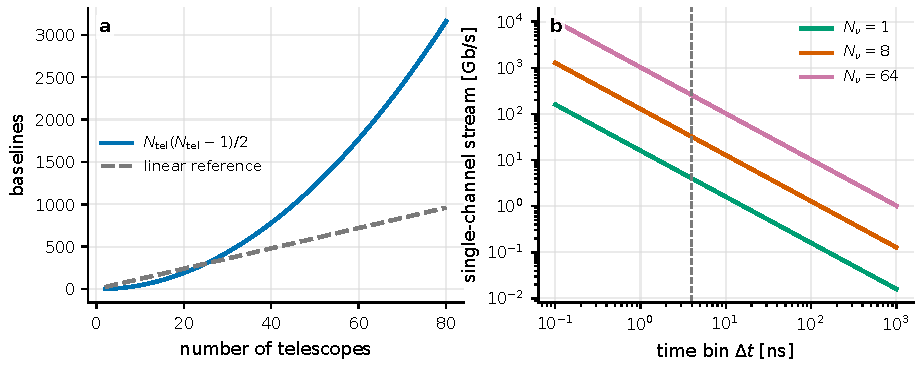
\includegraphics[width=0.96\linewidth]{figures/generated/chapter_20/ch20_correlator_scaling.pdf}
\caption{多望远镜相关器的两个标度。左图：基线数随望远镜数二次增长，阵列一扩就迅速增加相关任务。右图：单路数据流随时间箱变窄和光谱通道增多而上升；纳秒级采样加几十个光谱通道，已进入必须靠实时硬件或 GPU 处理的区域。}
\label{fig:e26-correlator}
\end{figure}

真正把这一节和前面区分开的，是\textbf{null test（零假设检验）}——而且它应该像结果图一样被认真评分，不是附录里的走过场。至少要做这几项：把第二路整体平移远大于 \(\tau_c\) 的时间，真实峰\textbf{必须消失}；盖上遮光片或没有星光时跑同样流程，电子学串扰\textbf{不该}冒出零延迟峰；把偏振或光谱通道打乱，只有物理上该相关的通道保留信号；把数据按时间切片，\(\hat g^{(2)}(0)-1\) 应该随积分时间按 \(T^{-1/2}\) 平稳收敛，而不是集中在某一小段时间里。这些检验直接决定一个峰能不能被解释成天体信号——Guerin 等人的桌面/在天实验、AQuEye/IquEye 的光子计数方案，以及现代切伦科夫阵列的强度干涉，都把它们当成结果的一部分 \citep{2017MNRAS.472.4126G,2016SPIE.9907E..0NZ,2021MNRAS.506.1585Z,2020NatAs...4.1164A}。\textbf{一句话的纪律}：一个通过了 null test 的小峰，比一个没通过 null test 的大峰值钱得多。

\section{数值演示 SPADE：信息不在最亮的像素里}
\label{sec:e26-spade}

现在换一个看似无关、实则同源的实验，呼应第 \ref{chap:e12} 章。前面用长基线去够高空间频率；这里的问题反过来：\textbf{已经成像了，两个点源挨得比点扩散函数还近，还能不能量出它们的分离？}直接成像的答案很沮丧，而模式排序（SPADE）会告诉你信息其实一直都在，只是没在你盯着的那几个亮像素里。

先建立画面。两个等亮、非相干的点源，分离 \(s\) 远小于点扩散函数（point spread function, PSF）宽度 \(\sigma\) 时，焦平面上的合成像几乎只是"稍微胖了一点点"。糟糕的是，像素强度对 \(s\) 的\textbf{导数}在 \(s\to0\) 时趋于零——你想估的参数几乎不改变你测的东西，于是费雪信息（Fisher information）塌向零。这就是\textbf{瑞利诅咒}（Rayleigh curse）在统计上的准确含义：不是"分辨不出"，而是"直接成像这个测量方式，把关于 \(s\) 的信息浪费掉了" \citep{2015Optic...2..646T,2016PhRvX...6c1033T}。

SPADE 换一种测量：不测像素强度，而是把光投影到一组\textbf{厄米–高斯模式}（Hermite--Gaussian modes）上，数每个模式里有几个光子。对高斯 PSF、等亮双点源，这是第 \ref{chap:e12} 章给出的已知结果——落到第 \(n\) 个模式的概率是泊松形的：
\begin{equation}
  p_n=e^{-\Gamma}\,\frac{\Gamma^{\,n}}{n!},\qquad
  \Gamma=\left(\frac{s}{4\sigma}\right)^{\!2}.
  \label{eq:e26-spade-prob}
\end{equation}
\begin{formulaexplain}
\(p_n\) 是一个光子被投影到第 \(n\) 个厄米–高斯模式的概率，\(n=0,1,2,\dots\) 是横向模式编号。\(\Gamma\) 是把分离与 PSF 宽度揉成的无量纲小量。分离越小 \(\Gamma\) 越小，绝大多数光子仍落在基模 \(n=0\)，但 \(n\ge1\) 的那点小概率对 \(s\) 极其敏感。
\end{formulaexplain}
落实符号：\(s\) 是角分离（与 \(\sigma\) 同用一种角单位或同一种焦面长度单位），\(\sigma\) 是 PSF 高斯宽度，\(\Gamma\)、\(p_n\) 无量纲。代数字：\(s=0.2\sigma\) 时 \(\Gamma=(0.2/4)^2=2.5\times10^{-3}\)，于是 \(p_1\approx\Gamma=2.5\times10^{-3}\)，一千个光子里才盼到两三个进 \(n=1\) 模式——但恰恰是这两三个光子扛着几乎全部关于 \(s\) 的信息。

为什么说信息没塌？把泊松概率式 \eqref{eq:e26-spade-prob} 的费雪信息一步步算出来。单个光子对参数 \(s\) 的费雪信息是
\[
  I_{\rm SPADE}(s)=\sum_{n}\frac{1}{p_n}\!\left(\frac{\partial p_n}{\partial s}\right)^{\!2}.
\]
利用泊松分布的一个标准事实——泊松均值 \(\Gamma\) 本身的费雪信息是 \(1/\Gamma\)，再用链式法则 \(I_s=(d\Gamma/ds)^2\cdot(1/\Gamma)\)。代 \(\Gamma=s^2/(16\sigma^2)\)，则 \(d\Gamma/ds=s/(8\sigma^2)\)，于是
\[
  I_{\rm SPADE}(s)=\frac{\big(s/8\sigma^2\big)^2}{s^2/(16\sigma^2)}
  =\frac{s^2/(64\sigma^4)}{s^2/(16\sigma^2)}=\frac{16\sigma^2}{64\sigma^4}=\frac{1}{4\sigma^2}.
\]
一步不跳，结果干净得惊人：\(I_{\rm SPADE}=1/(4\sigma^2)\)，\textbf{与分离 \(s\) 无关}——哪怕 \(s\to0\)，每个光子携带的信息也不衰减。对照之下，直接成像的费雪信息随 \(s\to0\) 塌向零。这就是 SPADE 越过瑞利诅咒的全部秘密。

\begin{figure}[tbp]
\centering
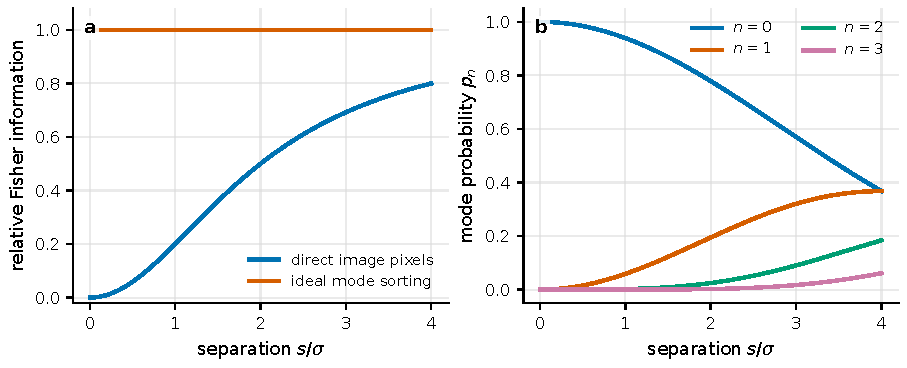
\includegraphics[width=0.96\linewidth]{figures/generated/chapter_20/ch20_spade_computational_experiment.pdf}
\caption{SPADE 计算实验。左图比较小分离处直接像素成像与理想模式排序的相对费雪信息：直接成像在 \(s/\sigma\ll1\) 时信息下降，模式排序保持接近常数。右图显示厄米–高斯模式概率，分离很小时高阶模式概率虽小但斜率非零，因此需要高稳定、低串扰的模式测量。}
\label{fig:e26-spade}
\end{figure}

\textbf{务必写进代码的坑}：上面那条漂亮的常数曲线是\textbf{理想}情形。真实系统里，模式基与真实 PSF 不完全匹配、中心定位有误差、有像差、有背景光——任何一点\textbf{模式串扰}（cross-talk）都会让本该干净的 \(n=1\) 模式漏进一点 \(n=0\) 的光，从而给费雪信息垫一块\textbf{信息地板}，把 \(s\to0\) 的优势削平。所以教学代码不该只画理想曲线，而要加一个可调的串扰参数，让学生看着信息地板随串扰升高而抬起。正因如此，SPADE 目前更适合当作计算实验和先导验证（pathfinder），而不是承诺下一代望远镜就能无损触及量子极限 \citep{2016OExpr..24.3684N,2017PhRvL.118g0801T}。

\section{综合项目：Type Ia 距离玩具模型如何串起整套误差预算}
\label{sec:e26-typeia}

最后一个项目把前面的零件拼成整机，也故意暴露玩具模型最容易掩盖的危险：角半径、速度、爆炸时间看起来只差一个比例常数，真实误差却来自\textbf{不同仪器、不同模型、不同历元}。这就是用膨胀光球法（expanding photosphere method）给 Type Ia 超新星测角直径距离的思路 \citep{2025PhRvD.111h3047K}。

物理链条是这样的：光谱模型给出光球膨胀速度 \(v_{\rm ph}(t)\)，强度干涉给出光球角半径 \(\theta_{\rm ph}(t)\)，两者一比就得到角直径距离：
\begin{equation}
  \theta_{\rm ph}(t)=\frac{R_{\rm ph}(t)}{D_A}\simeq\frac{v_{\rm ph}\,(t-t_0)}{D_A}.
  \label{eq:e26-typeia-theta}
\end{equation}
\begin{formulaexplain}
\(\theta_{\rm ph}\) 是光球角半径，\(R_{\rm ph}\) 是物理半径，\(D_A\) 是角直径距离，\(t_0\) 是爆炸时刻。若光球以近似恒定速度 \(v_{\rm ph}\) 膨胀，则物理半径约为速度乘时间；用它除以角半径，就把距离逼出来了。
\end{formulaexplain}
落实符号与量纲：\(v_{\rm ph}\) 单位 \(\mathrm{cm\,s^{-1}}\)，正常 Type Ia 早期约 \(8\times10^8\)–\(1.5\times10^9\,\mathrm{cm\,s^{-1}}\)；\(t-t_0\) 单位 s 或 d，强度干涉最感兴趣的是爆炸后几天到几十天；\(D_A\) 用 Mpc；\(\theta_{\rm ph}\) 通常几到几十 \(\mu\mathrm{as}\)。代真实数字：\(v_{\rm ph}=10^{9}\,\mathrm{cm\,s^{-1}}\)、\(t-t_0=15\,\mathrm{d}=1.30\times10^{6}\,\mathrm{s}\)，物理半径 \(R_{\rm ph}\approx1.30\times10^{15}\,\mathrm{cm}\)；再取 \(D_A=20\,\mathrm{Mpc}=6.17\times10^{25}\,\mathrm{cm}\)，
\[
  \theta_{\rm ph}\approx\frac{1.30\times10^{15}}{6.17\times10^{25}}\ \mathrm{rad}
  \approx2.1\times10^{-11}\,\mathrm{rad}\approx4.3\,\mu\mathrm{as}.
\]
在 \(\lambda=500\,\mathrm{nm}\) 下，这对应第一零点基线尺度 \(\lambda/\theta\sim24\,\mathrm{km}\)。若肯用整条可见度曲线而不只等第一零点，公里到十公里级基线仍有科学信息可挖——但误差预算会绷得极紧。

怎么把角半径和速度合成一个距离后验？写一个联合似然，同时惩罚"角半径预言"和"速度预言"的不一致：
\begin{equation}
  \ln{\cal L}(D_A)=
  -\frac12\sum_k\!\left[\frac{\hat\theta_k-v_{{\rm ph},k}(t_k-t_0)/D_A}{\sigma_{\theta,k}}\right]^2
  -\frac12\sum_k\!\left[\frac{\hat v_k-v_{{\rm ph},k}}{\sigma_{v,k}}\right]^2 .
  \label{eq:e26-typeia-like}
\end{equation}
\begin{formulaexplain}
\(D_A\) 是待估距离，\(\hat\theta_k\) 与 \(\hat v_k\) 是第 \(k\) 个历元测到的角半径与速度，\(\sigma_{\theta,k}\)、\(\sigma_{v,k}\) 是各自的误差。第一个和式管"角半径要和 \(v(t-t_0)/D_A\) 对上"，第二个和式管"速度模型要和测到的速度对上"。两项一起被最小化，才能同时约束 \(D_A\)。
\end{formulaexplain}
落实符号：\(\hat\theta_k\) 来自第 \(k\) 历元的 \(|V|^2\) 拟合（式 \eqref{eq:e26-v2-estimator}、\eqref{eq:e26-uniform-disk} 那套），单位 rad 或 \(\mu\mathrm{as}\)；\(\hat v_k\) 来自谱线速度或辐射转移模型，单位 \(\mathrm{cm\,s^{-1}}\)；\(\sigma_{\theta,k}\)、\(\sigma_{v,k}\) 各自\textbf{同时}包含统计误差和模型系统误差。\textbf{玩具模型最大的坑}正在这里：如果你偷懒只给 \(\hat\theta\) 加个 \(10\%\) 的高斯噪声，就会得到一个漂亮到失真的窄后验。真实项目必须让学生去动那些"看不见的旋钮"——变动爆炸时间 \(t_0\)、给速度加梯度、放进非球对称、换掉均匀圆盘换成有临边昏暗的亮度分布——然后看着后验一点点变宽。后验\textbf{应该}变宽，那才是诚实的误差预算。

\begin{figure}[tbp]
\centering
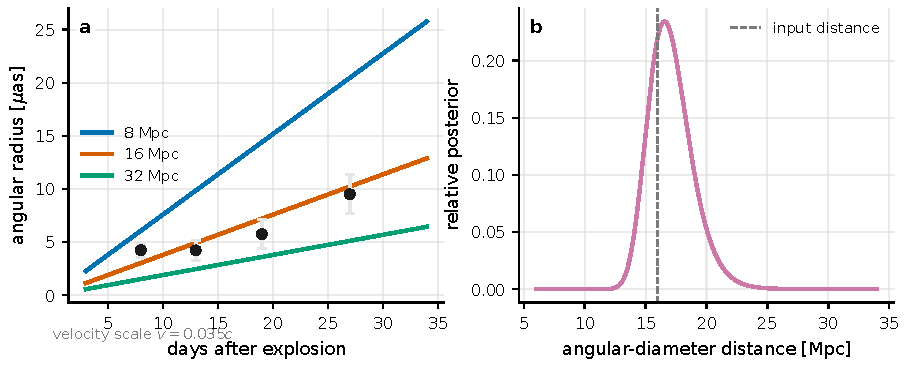
\includegraphics[width=0.96\linewidth]{figures/generated/chapter_20/ch20_typeia_distance_posterior.pdf}
\caption{Type Ia 超新星角直径距离玩具模型。左图用 \(v_{\rm ph}=0.035c\) 的简化膨胀模型，给出不同距离下角半径随时间的变化，并叠加模拟角半径测量；右图把这些角半径与速度模型合成 \(D_A\) 后验。真实分析要用辐射转移模型替代恒速球壳，并把非球对称、谱线形成层和基线覆盖都写进误差预算。}
\label{fig:e26-typeia}
\end{figure}

这五个项目连起来，正好是一条难度递进的课程线：先用 LED、伪热光、激光测 \(g^{(2)}(\tau)\)，验证泊松与聚束；再在同一份事件表上练 time-shift 背景、质量筛选和 \(T^{-1/2}\) 收敛；进入空间相干后拟合均匀圆盘和双星 \(|V|^2\)，体会基线覆盖的作用；然后做 SPADE，看费雪信息如何逃过瑞利诅咒，又如何被串扰按回地板；最后用 Type Ia 玩具模型把角半径、速度、爆炸时间的不确定性一起传播。每个项目的交付物都一样朴素：一份事件表说明、一个能跑的脚本、一组图、一份点了真实文献的短报告，以及\textbf{至少两个 null test}。记住本章反复出现的那句话——代码能跑只是第一关；说不清时间基准、\(\beta\) 标定、串扰矩阵或系统误差的图，可以生成，但不能当成一次天文测量。

\section*{本章要点}
\addcontentsline{toc}{section}{本章要点}

\begin{itemize}
  \item \textbf{一切从事件表开始。}每个光子留下时间、通道、偏振、质量标记；光变曲线只是它的一个有损投影（式 \eqref{eq:e26-binned-count}）。先分箱，就永远回不去了。
  \item \textbf{泊松的签名是方差等于均值。}用法诺因子 \(F=\operatorname{Var}/\langle N\rangle\to1\) 检验散粒噪声（式 \eqref{eq:e26-fano}）；\(F<1\) 常是死时间伪装的反聚束，不是新物理。
  \item \textbf{聚束靠符合超额被看见，但会被稀释。}\(\hat g^{(2)}\) 用 time-shift 背景归一化（式 \eqref{eq:e26-g2-estimator}）；相干时间远小于响应宽度时，热光峰按 \(\tau_c/\Delta\tau\) 缩小到 \(10^{-5}\) 量级。
  \item \textbf{可见度是天体的傅里叶指纹。}\(|V|^2\) 从 \(\hat g^{(2)}(0)-1\) 除以仪器对比度 \(\beta\) 得到（式 \eqref{eq:e26-v2-estimator}）；\(\beta\) 在分母，标定误差被直接放大。均匀圆盘第一零点 \(B_{\rm null}\approx1.22\lambda/\theta\)（式 \eqref{eq:e26-uniform-disk}），\(1\,\mathrm{mas}\) 亮星约在百米基线。
  \item \textbf{多基线、多历元是为了拆简并。}双星的振荡半幅 \(2\rho/(1+\rho)^2\)（式 \eqref{eq:e26-binary}）随伴星变暗而变浅；单方向的 uv 覆盖会给出被拉长的误导性误差椭圆。
  \item \textbf{相关器一半的价值是 null test。}时间平移、遮光、通道打乱、\(T^{-1/2}\) 收敛都要像结果一样评分；数据率标度（式 \eqref{eq:e26-datarate}）解释了为何非要实时硬件。
  \item \textbf{SPADE 把信息从亮像素里解放出来。}模式概率是泊松形（式 \eqref{eq:e26-spade-prob}），费雪信息 \(1/(4\sigma^2)\) 与分离无关；但串扰会垫起信息地板，理想曲线不可轻信。
  \item \textbf{综合项目考的是误差预算，不是拟合。}Type Ia 距离玩具模型（式 \eqref{eq:e26-typeia-theta}、\eqref{eq:e26-typeia-like}）里，后验\textbf{应该}在你放进真实系统误差后变宽；不变宽，说明你还没把危险放进来。
\end{itemize}

\medskip
\noindent\textbf{想一想：}(1) 你测到 \(F=0.7\)，请给出至少两种物理上不同的解释，并各设计一个能把它们区分开的实验。(2) 若把双星的伴星通量比从 \(\rho=0.3\) 降到 \(\rho=0.05\)，要维持同样的振荡显著性，随机符合数 \(H\) 大致要增大多少倍？(3) 在 SPADE 里加入 \(1\%\) 的模式串扰，信息地板会把可分辨的最小 \(s/\sigma\) 顶到多大量级？
